\begin{figure}[H]
    \begin{subfigure}[t]{.35\textwidth}
        \caption{}
        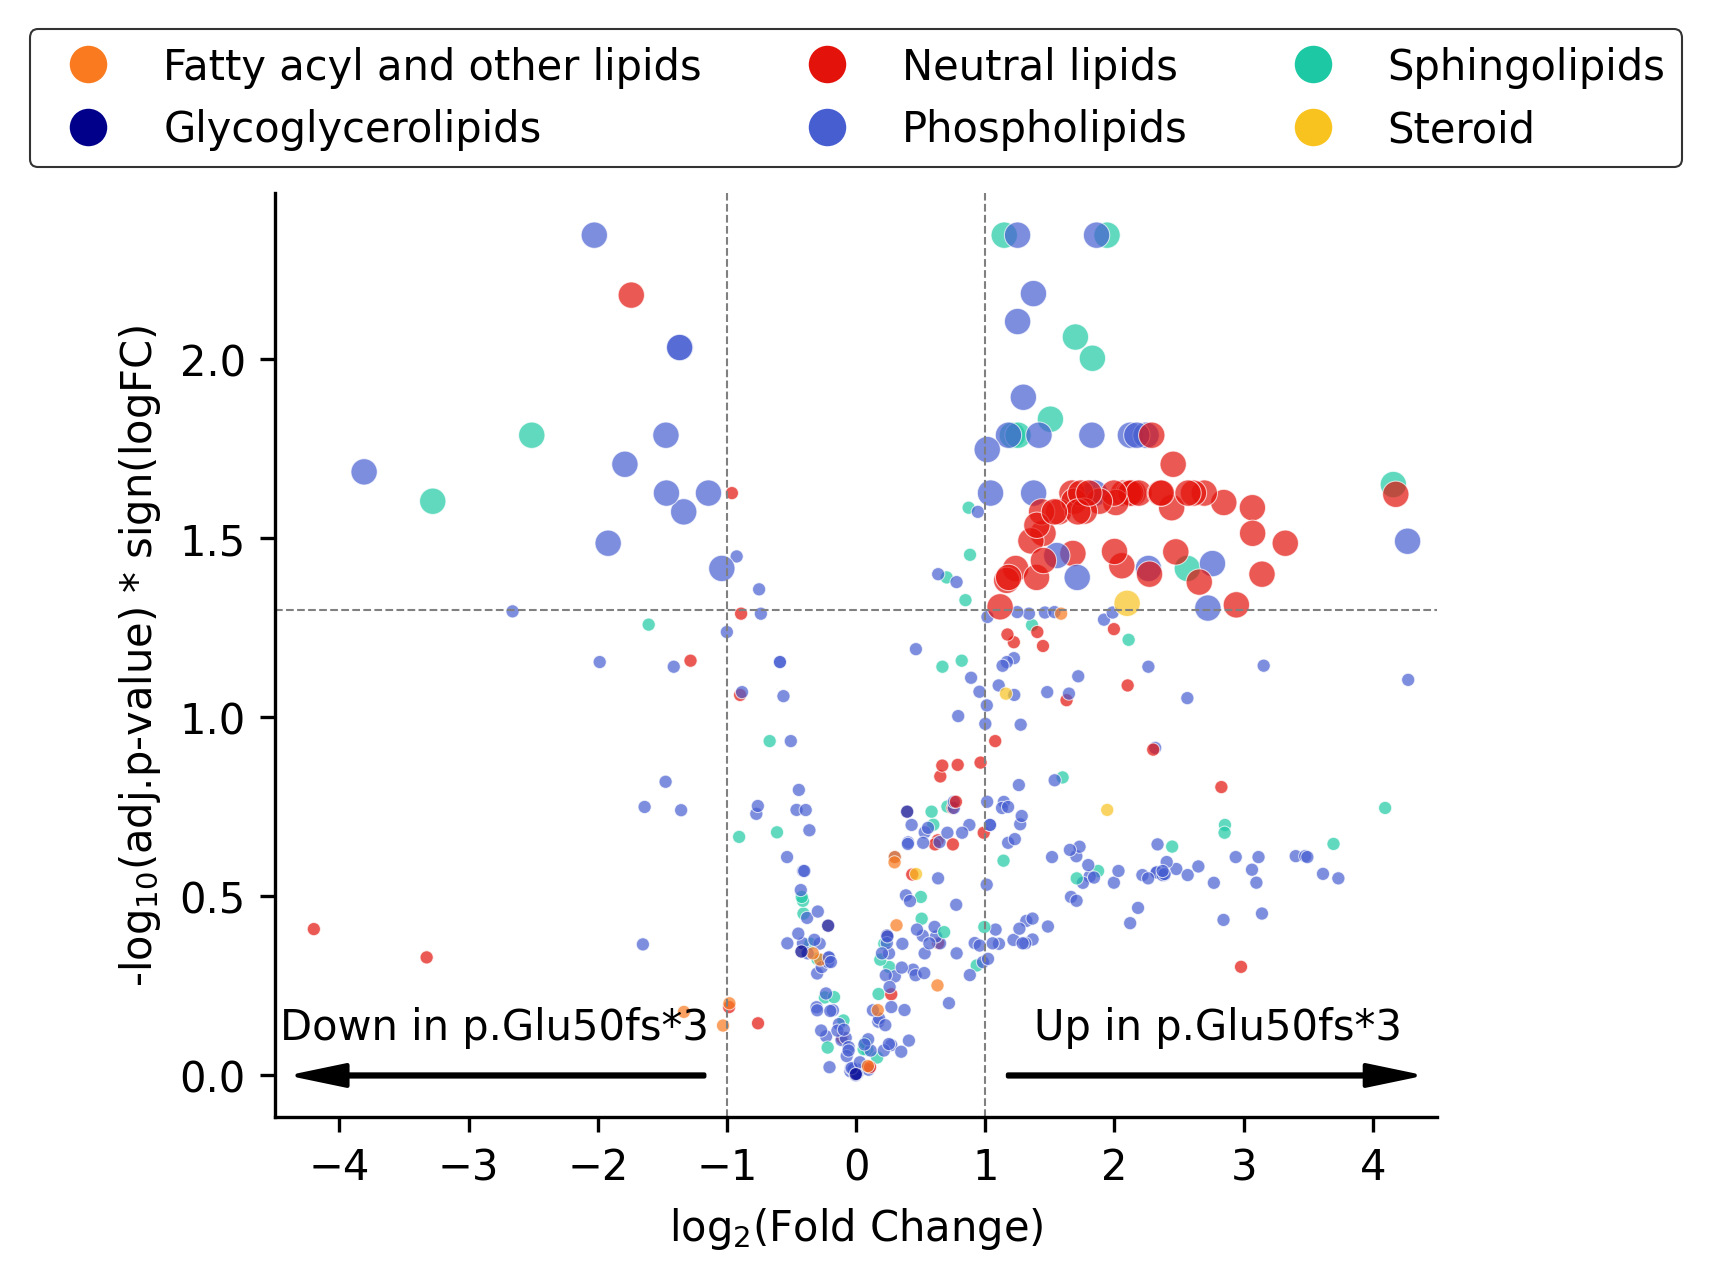
\includegraphics[width=\textwidth]{./main_plots/iN_lipids_overview.png}        
    \end{subfigure} 
    \begin{subfigure}[t]{.35\textwidth}
        \caption{}
        \includegraphics[width=\textwidth]{./main_plots/lipids_table.png}        
    \end{subfigure} 
    \begin{subfigure}[t]{.35\textwidth}
        \caption{}
        \includegraphics[width=\textwidth]{./main_plots/tg_carbons.png}        
    \end{subfigure} 
    \begin{subfigure}[t]{.35\textwidth}
        \caption{}
        \includegraphics[width=\textwidth]{./main_plots/G2_PC_volcano_sat.png}        
    \end{subfigure} 
    \begin{subfigure}[t]{.35\textwidth}
        \caption{}
        \includegraphics[width=\textwidth]{./main_plots/G2_PC_volcano_unsat.png}        
    \end{subfigure} 
    \begin{subfigure}[t]{.35\textwidth}
        \caption{}
        \includegraphics[width=\textwidth]{./main_plots/pc_unsat.png}        
    \end{subfigure} 
    \begin{subfigure}[t]{.35\textwidth}
        \caption{}
        \includegraphics[width=\textwidth]{./main_plots/lipids_table_y622.png}        
    \end{subfigure}
    \begin{subfigure}[t]{.35\textwidth}
        \caption{}
        \includegraphics[width=\textwidth]{./main_plots/Y622_PC_volcano_sat.png}        
    \end{subfigure} 
    \begin{subfigure}[t]{.35\textwidth}
        \caption{}
        \includegraphics[width=\textwidth]{./main_plots/tg_carbons_y622.png}        
    \end{subfigure} 
    \begin{subfigure}[t]{.35\textwidth}
        \caption{}
        \includegraphics[width=\textwidth]{./main_plots/pc_unsat_y622.png}        
    \end{subfigure} 
    \begin{subfigure}[t]{.2\textwidth}
        \caption{}
        \includegraphics[width=\textwidth]{./extended_plots/g2_lpcat.png}        
    \end{subfigure} 
    \begin{subfigure}[t]{.2\textwidth}
        \caption{}
        \includegraphics[width=\textwidth]{./extended_plots/y622_lpcat.png}        
    \end{subfigure} 
    \caption{
        \textbf{ABCA7 LoF Neurons Have Neutral Lipid Accumulation and Phospholipid Imbalances.}\\
    }
    \label{fig:main_lipids}
\end{figure}
\begin{itemize}
    \item[\textbf{(A)}] Volcano plot indicating perturbed lipid species by LCMS in p.Glu50fs*3 vs. WT iNs (p-adjusted < 0.05 and |logFC|>1) colored by lipid class.
    \item[\textbf{(B)}] Significantly perturbed lipid species from (A) broken down by lipid sub class.
    \item[\textbf{(C)}] Distribution of triglyceride fold changes by chain lengths and saturation.
    \item[\textbf{(D)}] Volcano plot indicating perturbed phosphatidylcholine species that contain saturated or monounsaturated fatty acids (SFA; MUFA). 
    \item[\textbf{(E)}] Volcano plot indicating perturbed phosphatidylcholine species that contain polyunsaturated fatty acids (PUFA).
    \item[\textbf{(F)}] Distribution of phosphatidylcholine fold changes by chain lengths and saturation. 
    \item[\textbf{(G)}] Table indicating perturbed lipid species by lipid subclass in p.Tyr622* vs. WT iNs.
    \item[\textbf{(H)}] Showing all lipid species from (G) colored; phosphatidylcholine species are highlighted in blue.
    \item[\textbf{(I,J)}] Same as C,F for p.Tyr622* vs. WT iNs.
    \item[\textbf{(K,L)}] LPCAT gene changes in p.Tyr622* vs. WT iNs and p.Glu50fs*3 vs. WT iNs (mRNA).
\end{itemize}